\documentclass{article}
\usepackage{graphicx} % Required for inserting images
%Welcome :)

\documentclass{article}

% Basic document formatting
\usepackage[utf8]{inputenc}     % Input encoding
\usepackage[T1]{fontenc}        % Font encoding
\usepackage{lmodern}            % Modern LaTeX fonts
\usepackage{geometry}           % Set page margins
\geometry{a4paper, total={170mm,257mm}, left=20mm, top=20mm} 
\usepackage{float}              % Handling of floating elements
\usepackage{fancyhdr}           % Fancy headers
\usepackage{lastpage}           % use \pageref{LastPage} to make page x of y footers
\setlength{\parindent}{0pt}     % No \noindent

% Figures
\usepackage{graphicx}           % For including images
\usepackage{caption}            % Using the caption package
\usepackage{wrapfig}            % For including Wrap Figures
\usepackage{subcaption}         % For subfigures within a figure environment
\usepackage{pgfplots}           % Drawing plots
\usepackage{pgf-pie}            % For creating pie charts
\captionsetup[figure]{labelfont=bf}
\captionsetup[table]{labelfont=bf}
\usepackage{asymptote}          % Zum Zeichnen verschiedener Plots 
\usepackage{pdfpages}           % Zum Einfügen ganzer PDFs

% Colorboxes
\usepackage[skins]{tcolorbox}   % Color Boxes

% Tables and long tables
\usepackage{tabularx}           % Advanced table features
\usepackage{longtable}          % For tables that span multiple pages
\usepackage{multirow}           % Allows for multirow cells in tables
\usepackage{booktabs}           % For professional-quality tables

% Math packages
\usepackage{amsmath}            % Enhanced mathematical formatting
\usepackage{amssymb}            % Extended symbol collection
\usepackage{amsfonts}           % Mathematical fonts
\usepackage[version=4]{mhchem}  % Chemische Formeln
\usepackage{mathtools}          % Mathematical tools to supplement amsmath
\numberwithin{equation}{section} % Numbers Equations with chapters
\usepackage{siunitx}            % Makes SI-Units

% Code display
\usepackage{listings}           % For displaying code
\usepackage{xcolor}             % For coloring code
\lstdefinestyle{mystyle}{
    backgroundcolor=\color{backcolour},   
    commentstyle=\color{codegreen},
    keywordstyle=\color{ao},
    numberstyle=\tiny\color{codegray},
    basicstyle=\ttfamily\footnotesize,
    breakatwhitespace=false,         
    breaklines=true,                 
    captionpos=b,                    
    keepspaces=true,                 
    numbers=left,                    
    numbersep=5pt,                  
    showspaces=false,                
    showstringspaces=false,
    showtabs=false,                  
    tabsize=2
}
\lstset{style=mystyle}

% Custom Colours
\definecolor{LightCyan}{rgb}{0.88,1,1}
\definecolor{dkgreen}{rgb}{0,0.6,0}
\definecolor{gray}{rgb}{0.5,0.5,0.5}
\definecolor{mauve}{rgb}{0.58,0,0.82}
\definecolor{codegreen}{rgb}{0,0.6,0}
\definecolor{codegray}{rgb}{0.5,0.5,0.5}
\definecolor{ao}{rgb}{0.0, 0.0, 1.0}
\definecolor{backcolour}{rgb}{0.95,0.95,0.92}

% Referencing
\usepackage[style=numeric, backend=biber, sorting=none]{biblatex} % Imports biblatex package
\addbibresource{MAIN.bib} %Import the bibliography file
\DeclareFieldFormat{labelnumberwidth}{\mkbibbrackets{#1}} %ensure that the label numbers in the bibliography are enclosed in brackets.
\usepackage{xurl}

% Hyperlinks in the document
\usepackage{hyperref}           % For adding hyperlinks


\begin{document}

\vspace{-4cm}

\includegraphics[width=0.25\linewidth]{Graphics/VCS-Logo.png}

\vspace{-1.5cm}
\begin{flushright}
\parbox[r]{5cm}{Zurich, \today}
\end{flushright}

\vspace{1.5cm}
\begin{center}
\textbf{\LARGE{Walk \& Talk mit der VCS}} \\
\vspace{0.5cm}
\Large
VCS - Vereinigung der Studierenden der Chemie-, Biochemie – Chemische Biologie, 
Chemieingenieurwissenschaften und interdisziplinären Naturwissenschaften
\end{center}

\section{Marco Ponts Teaching Award}
Die VCS hat in Absprache mit dem D-CHAB und VAC ein Konzept für einen Teaching Award initiiert. Der Award wird zu Ehren von Marco Ponts verliehen, einem ehemaligen, sehr geschätzten Studenten, der das studentische Leben für viele wesentlich bereichert hat. \\ 

Ebenfalls im Hinblick auf die Umsetzung von PAKETH sehen wir die Chance Studierende im Semester besser mitzunehmen durch gute Übungsstunden, die von Teaching Assistants durchgeführt werden. 
Für die Gewinner*innen verleihen wir einen physischen Preis und sind in Rücksprache mit dem D-CHAB über ein Preisgeld. 


\section{PAKETH}

\subsection{Weniger Zeit im Semester}

Durch die Umstellung des Curriculums durch PAKETH, wird der wesentliche Lernaufwand der Studierenden in das Semester verschoben, wohingegen zur Zeit - gerade am D-CHAB durch die zeitintensiven Praktika unter dem Semester - auch ein wesentlicher Teil des Lernens im Zwischensemester liegt. Wir und viele Studierende in unserem Departement teilen die Sorge, dass einerseits durch die deutlich verkürzte Lernphase die Prüfungsvorbereitungskurse (PVKs) wegfallen werden und andererseits unter dem Semester kaum noch Zeit für andere Tätigkeiten wie ehrenamtliches Engagement in den Fachvereinen oder die Arbeit als Teaching Assistant bleibt. Bei den PVKs bietet die VCS für nahezu jede Pflichtprüfung der ersten beiden Studienjahre drei- bis fünftägige Kurse in den ersten vier Wochen der Lernphase an. Die PVKs werden von den Teilnehmenden in der Regel äusserst positiv bewertet. Ausserdem werden die TA-Stellen am D-CHAB in den ersten beiden Studienjahren vorrangig von Studierenden besetzt und eher weniger von Doktorierenden. Wir sind der Ansicht, dass die Arbeit als TA mit dem gesteigerten Arbeitspensum unter dem Semester kaum noch möglich sein wird. Ein ähnliches Problem ist dort auch das Engagement im Fachvereinsvorstand, denn diese Tätigkeit ist ebenfalls mit einem erheblichen Zeitaufwand verbunden.

% \subsection{Bonussysteme}
%Bereits jetzt gibt es schon Systeme, die Studierende, die im Semester eine Vorlesung verfolgen, belohnen sollen. In unseren Studiengängen wird ein Bonus durch Abgabe von Übungen in der Physik I und II Vorlesung angeboten. \\
%Ein anderes System ist in der Informatik I Vorlesung implementiert. Es gibt 2-3 wöchige Aufgaben, die ein fünftel der Schlussnote ausmachen. Das "nicht-abgeben" würde hier effektiv zu einer Verschlechterung der Endnote führen. \\
%Allein im Vergleich zwischen diesen Methoden gibt es eine Prioritisierung für die zweite Variante, bei der das "nicht-abgeben" eine drastischere Konsequenz beinhaltet. Uns und dem D-CHAB ist es wichtig, dass Studierende im Semester den Stoff der Vorlesungen verfolgen, jedoch bereitet uns die Sinnhaftigkeit der Bonussysteme Sorge. Denn die Dozent*innen wissen, dass Studierende die Fächer mit Bonusangebot prioritisieren 

\subsection{Abmeldefrist von Prüfungen}
Wir glauben, dass eine möglichst späte Abmeldung von den Prüfungen unseren Studierenden eine wichtige Freiheit erlaubt. Bereits am Anfang des Semesters entscheiden zu müssen, welche Prüfungen man einige Monate später ablegen wird, ist eine große Herausforderung. Viele Studierende brauchen mehr als drei Wochen, um abschätzen zu können, ob sie die Prüfungen während der Prüfungssession ablegen möchten. Besonders im dritten Jahr Chemieingenieurwissenschaften (CI) ist aufgefallen, dass von zwei Blöcken des Herbstsemesters viele Studierende einen schieben. \\

Wir sehen einen großen Vorteil darin, die Abmeldung von einer Lerneinheit (und ihrer Prüfung) soweit wie möglich nach hinten zu verschieben, da es Studierende ermutigt, auch schwierige Fächer/Blöcke zu belegen. Es ist durchaus denkbar, dass sich weniger Studierende das zutrauen, wenn die Möglichkeit der Abmeldung der Prüfungen wegfällt. 

\subsection{Video-Aufzeichnungen}
Um während des Semesters bei den Lehrveranstaltungen möglichst gut dabeizubleiben, empfinden es viele Studierende als große Hilfe, wenn Sie Vorlesungen nachschauen können, insofern diese aufgezeichnet werden.\\
Zudem kommt es insbesondere bei Studierenden der Interdisziplinären Naturwissenschaften (N-lern) sehr häufig, sowie bei anderen Studiengängen gelgentlich zu Fächerüberschneidungen, bei welchen Videoaufzeichnungen wesentlich für das ausführliche Nacharbeiten der Fächer sind.\\ 
Ebenso trifft dies auf den Krankheitsfall zu - auch mit Hinblick auf die mehr in den Fokus rückende mentale Gesundhet der Studierenden kann es nur von Vorteil sein, verlässlich zu wissen, dass Vorlesungen jederzeit mit Video-Aufzeichnung nachgearbeitet werden können. \\ 
Daher möchten wir mit Hinblick auf PAKETH anbringen, dass wir ein verpflichtendes Aufzeichnen aller Vorlesungen sehr begrüssen würden.

\subsection{AOCP II Laborplatzvergabe}
Die Platzvergabe im AOCP II Labor empfinden wir als ungerecht. Die Vergabe von Plätzen für das Labor 529-0129-00 P (Inorganic and Organic Chemistry II) im Herbstsemester erfolgt nach Basisprüfungsnoten, da die Platzanzahl beschränkt ist. Für Studierende der Chemie (CH) und Chemieingenieurwissenschaften (CI) ist das Praktikum eine Pflichtveranstaltung und muss absolviert werden. 

\begin{figure}[H]
    \centering
    
\includegraphics[width=1.05\linewidth]{Graphics/Screenshot 2025-03-11 at 16.18.40.png}
    \caption{Auszug aus dem VVZ}
    \label{fig:enter-label}
\end{figure}

Im \href{https://www.vvz.ethz.ch/Vorlesungsverzeichnis/lerneinheit.view?semkez=2024W&ansicht=ALLE&lerneinheitId=182740&lang=de}{Vorlesungsverzeichnis} (VVZ) und nach Angaben von betroffenen Studierenden werden die Plätze nach der Basisprüfungsnote vergeben. Die Problematik besteht darin, dass sich neben den Studierenden der CH und CI auch Studierende der Interdisziplinären Naturwissenschaften für das Praktikum bewerben. Insgesamt gibt es nicht genug Plätze und manche für Studierende der CH und CI, für die das Praktikum Pflichtbestandteil des Studiums ist, gibt es keinen Platz, obwohl sie die Basisprüfung bestanden haben.

\begin{figure}[H]
    \centering
    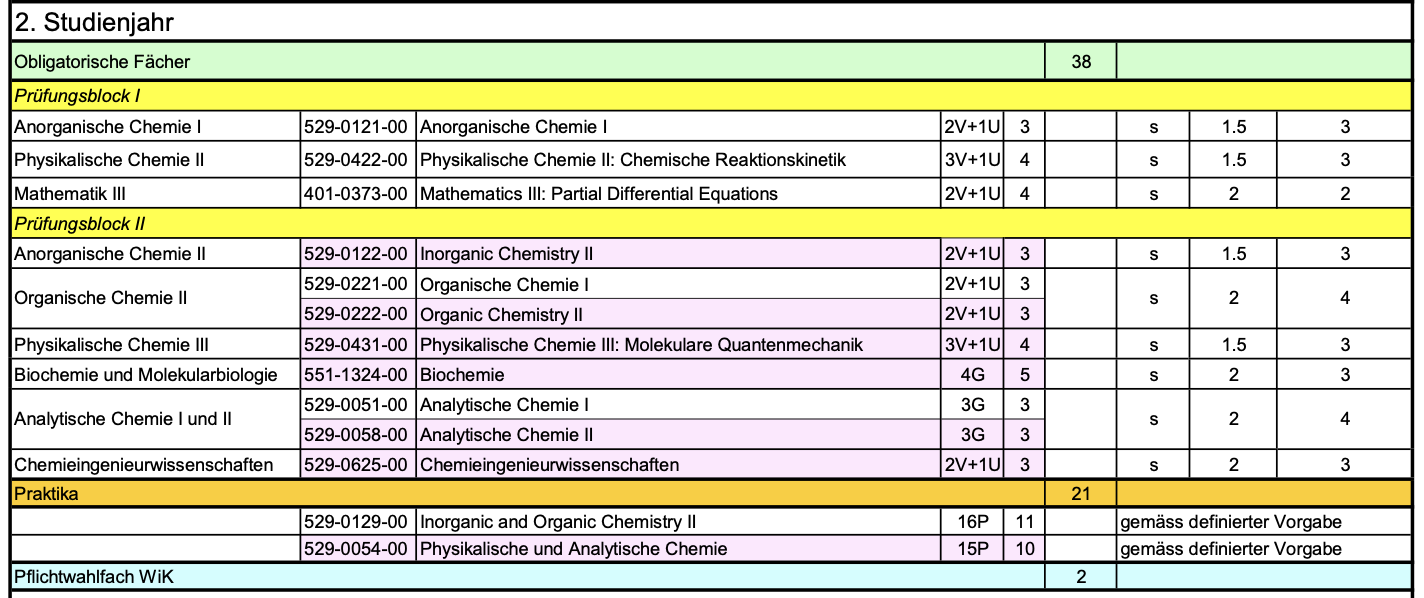
\includegraphics[width=0.9\linewidth]{Graphics/Screenshot 2025-03-11 at 16.23.07.png}
    \caption{Auszug aus der Übersicht des CH Bachelor Studiums}
    \label{fig:enter-label}
\end{figure}

Wir finden, dass die Platzvergabe unfair ist, da Studierende der CH und CI, die keinen Laborplatz bekommen, ein Semester länger als vorgesehene Regelstudienzeit studieren müssen, um alle drei Praktika der Herbstsemester absolvieren zu können. In unseren Augen ist das Praktikum zwar auch wichtig für Studierende der Interdisziplinären Naturwissenschaften, die sich ebenfalls in diese Richtung spezialisieren möchten, doch sollten entweder die CH und CI Studierenden priorisiert werden oder mehr Laborplätze zu Verfügung gestellt werden, um die Ungerechtigkeit aufzuheben. Eine weitere Möglichkeit dieses Problem zu lösen ist auch, das Praktikum ebenfalls im Frühjahrssemester für eine kleinere Gruppe von Studierenden (wie den Nlern) anzubieten, da die Laborplätze im FS nicht genutzt werden. Dieses Problem ist kein neues, denn es wurde bereits in der UK-C im Oktober 2009 darauf hingewiesen, dass das Praktikum seine Kapazitätsgrenze erreicht hatte und seitdem mehrfach darauf hingewiesen, dass es kein Platzproblem gäbe.

\subsection{Service Lectures – Biochemie (D-BIOL)}

Im D-CHAB gibt es jedes Jahr aufs Neue Beschwerden über eine spezifische Service Lecture des D-BIOL: die Vorlesung "Biochemie". Diese Vorlesung ist ein wiederkehrender Streitpunkt, der sowohl in UKs als auch zwischen den Departementen diskutiert wurde.

Das Problem besteht darin, dass diese Vorlesung vom D-BIOL für Studierende der Biologie, Pharmazie, Biochemie, Chemie und Chemieingenieurwissenschaften angeboten wird und bei allen als Teil eines Prüfungsblocks im zweiten Studienjahr geprüft wird. Sowohl die Departemente als auch wir Studierenden sind uns einig, dass die Gestaltung der Vorlesung und der Prüfung insbesondere für Studierende der Chemie und Chemieingenieurwissenschaften nicht fair ist. Der Grund: Diese beiden Studiengänge haben die Vorlesungen "Grundlagen der Biologie I" und "Grundlagen der Biologie II" im ersten Studienjahr nicht belegt. Alle anderen Studiengänge hatten diese Vorlesungen als Teil ihres Basisprüfungsblocks und damit die erforderlichen Grundlagen bereits erworben.  

Die VCS hat versucht, eine Veränderung zu bewirken, um diese Ungerechtigkeit zu korrigieren. Ein Vorschlag war, die Prüfungen für die beiden Studierendengruppen separat zu bewerten:

\begin{itemize}
    \item \textbf{Kohorte 1}: Studierende der Biologie, Pharmazie, Biochemie und Interdisziplinären Naturwissenschaften
    \item \textbf{Kohorte 2}: Studierende der Chemie und Chemieingenieurwissenschaften
\end{itemize}

Eine weitere Überlegung war, einen Teil der Biochemie-Vorlesung durch Inhalte aus "Grundlagen der Biologie I" zu ersetzen, um für die Studierenden der zweiten Kohorte die notwendigen Grundlagen zu schaffen. Dadurch könnten die Prüfungen der beiden Kohorten ebenfalls voneinander entkoppelt werden.  

Da es sich um eine Service Lecture handelt, liegt der Handlungsspielraum beim D-BIOL. Obwohl das Departement das Problem anerkennt und bedauert, sieht es keinen Anlass, Änderungen vorzunehmen.  

Die VCS möchte sich insbesondere im Rahmen der Implementierung von PAKETH dafür einsetzen, dass diese Problematik gelöst wird. Das D-BIOL sieht derzeit nur eine Lösung darin, dass das D-CHAB seine eigene Biochemie-Vorlesung anbietet. Dass eine solche Trennung möglich ist, zeigt die Situation bei der Mikrobiologie-Vorlesung:

\begin{itemize}
    \item \textbf{551-0313-00L} \textit{Microbiology (D-BIOL)} für Studierende der Biologie, Pharmazie (Wahlfach) und Biochemie (Wahlfach)
    \item \textbf{752-4001-00L} \textit{Mikrobiologie (D-CHAB)} für Studierende der Chemieingenieurwissenschaften, Interdisziplinären Naturwissenschaften (Wahlfach), Agrarwissenschaften, Umweltingenieurwissenschaften, Lebensmittelwissenschaften und Ernährung, Umweltnaturwissenschaften
\end{itemize}

Wir sind der Meinung, dass es höchste Zeit ist, diese Ungerechtigkeit zu beseitigen. Für uns sind verschiedene Lösungsansätze denkbar, doch es muss noch vor der Einführung von PAKETH eine Lösung gefunden werden. Andernfalls wird sich die bestehende Lücke in den Grundlagen für Studierende der Chemie und Chemieingenieurwissenschaften weiterhin in den Noten und Bestehensquoten widerspiegeln.


\subsection{Kreditpunktesystem}
Bisher belegen die Studierenden der VCS im Basisjahr verpflichtend 12-13 Fächer und zusätzlich Praktika, welche in der bisherigen Basisprüfung ohne Split zu 8-9 Prüfungen im Sommer zusammengefasst wurden. Dies war für viele Studierende nur mit einem sehr lernintensiven Sommer zu schaffen. Angesichts der gerade einmal zwei Wochen langen Lernzeit, die Stand PAKETH Konzeptbereinigung (Dezember 2024) vor der Repititionswoche und der Sessionsprüfungsphase geplant sind, haben wir Bedenken, wie realistisch eine solche Lernleistung für die Studierenden in so kurzer Zeit werden kann.\\ 
Vor allem, da es dem Empfinden vieler Studierenden nach derzeit grosse Dissonanz zwischen dem erwarteten Arbeitsaufwand pro Kreditpunkt an verschiedenen Departementen gibt, möchten wir grosses Augenmerk auf die Evaluation des Arbeitsaufwands und eventuelle Neuverteilung der ECTS auf die Module legen.\\ 
Es schliesst sich hier auch die hypothetische Frage an, wie damit umgegangen werden sollte, falls sich im Laufe der Evaluation der bestehenden Lerneinheiten die Summe der ECTS in Pflichtmodulen eines Bachelor-Studiums auf mehr als 180 belaufen würde. Hier interessieren wir uns sehr für Ihre Einschätzung.


\subsection{Orientierungssemester}
Wir möchten in der Diskussion um das Orientierungssemester gerne einbringen, dass wir dieses als sehr wichtig für Studierende empfinden. Das Orientierungssemester ist gedacht für Studierende, die zweimal einen Prüfungsblock nicht bestanden haben und somit aus dem Studienfach ausgeschlossen sind. Das Orientierungssemester bietet Studierenden die Möglichkeit, ein Semester nach dem Nicht-Bestehen weiter zu studieren und Fächer zu belegen, die außerhalb ihres vorherigen Fachgebiets liegen. Dies dient der Orientierung und bietet die Chance, Studierende nicht direkt aus dem Universitätskontext auszuschließen.\\

In Anbetracht der Tatsache, dass die Prüfungsergebnisse erst einige Tage vor Beginn des neuen Semesters veröffentlicht werden, ist es uns kaum ersichtlich, wie zu erwarten ist, dass eine Person sich so schnell auf einen neuen Studiengang/kein Studium entscheiden kann.\\

Uns ist wichtig, dass das Orientierungssemester weiterhin eine Möglichkeit bleibt, zumindest für die Studierenden, die nach dem zweiten oder dritten Jahr aus dem Studiengang ausgeschlossen werden, da sie der Ausschluss vom Studiengang besonders trifft.

\end{document}